\section{Cimentaciones superficiales} % (fold)
\label{sec:parte_2}


\question{Indica las principales hipotésis del método edométrico para el cálculo de asientos de consolidación y describe brevemente su grado de validez.}{
	Hipótesis:
	\begin{enumerate}
		\item Cálculo de $\sigma_v$ por elasticidad.
		\item $\Delta u = \Delta \sigma_v = \Delta \sigma_v^{’}$, el aumento de presión interna es igual al aumente de presión vertical.
		\item Las tensiones totales se mantienen invariantes a lo largo de la consolidación.
	\end{enumerate}
	Es válido (muy usado) aunque la segunda hipótesis se distancia de la realidad.
	\begin{myrem}[Skempton-Bjerrum]
		Intenta mejorar el efecto de la segunda hipótesis.
	\end{myrem}
}


\question{Calcular FS de la cimentación cuadrada de la Figure~\ref{fig:cimen} en condiciones no drenadas utilizando carga neta. Comenta el resultado.}{
	Al estar en situación no drenada tenemos:
	\[
		q_r = C_u N_c + q
	\]
	\begin{figure}[H]
		\centering
		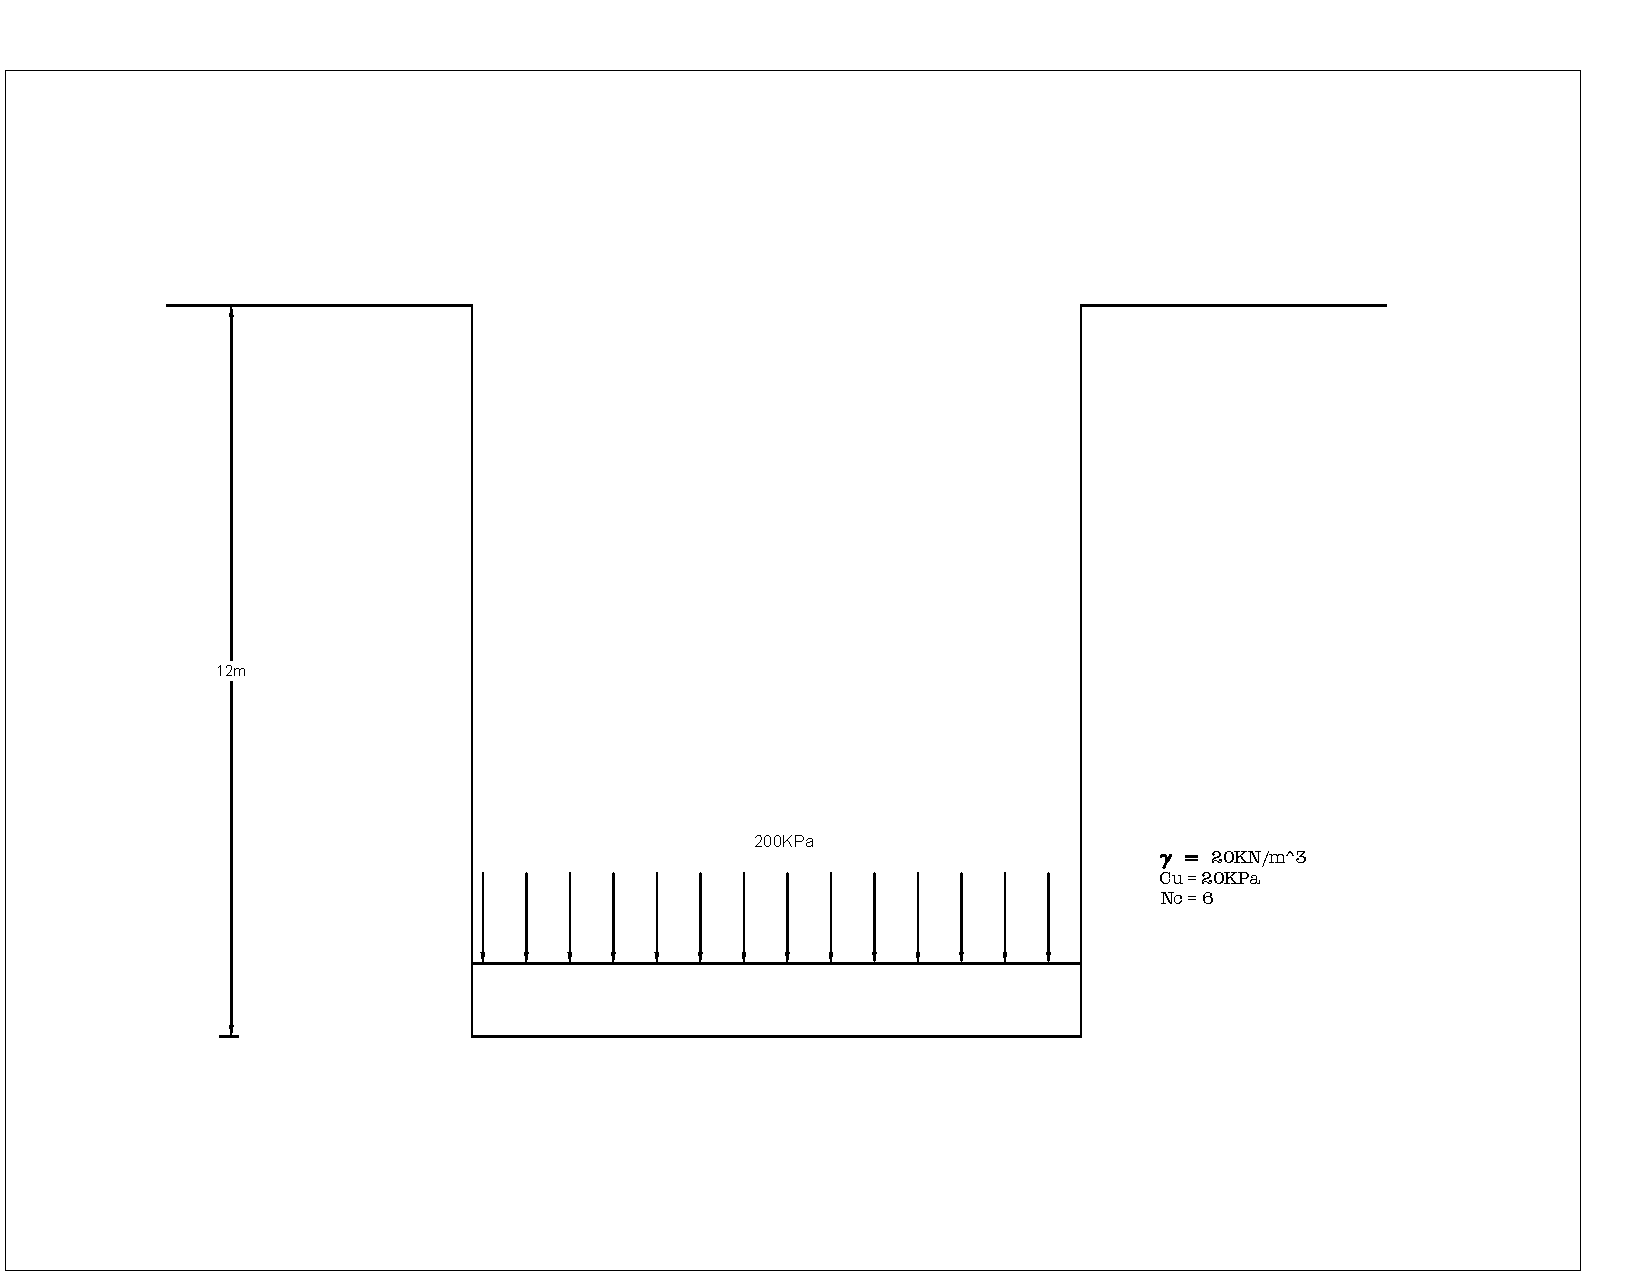
\includegraphics[width=0.9\textwidth]{img/capacidad_portante}
		\caption{Cimentación cuadrada}
		\label{fig:cimen}
	\end{figure}

	Tenemos (aplicando carga neta):
	\[
		FS = \frac{q_r - q}{q_{ad}-q} = \frac{360-240}{200 - 240} <0
	\]


	Lo cual es lógico ya que si analizamos la carga que este terreno soportaba antes de excavar observamos que era superior. Luego no hay razón de dudar de la estabilidad de esta cimentación.

	\begin{myrem}[FS real]
		Al calcular sin carga neta obtenemos
		\[
			FS = \frac{q_r }{q_{ad}} = \frac{360}{200} \approx 1,8
		\]
		Lo cual es incoherente con lo previamente comentado.
	\end{myrem}
}



\question{El asiento de una placa circular rígida sobre un semiespacio elástico homogéneo se expresa como $s=\frac{1-\mu^2}{2}\frac{P}{aE}$, donde s es el asiento, P la carga total aplicada, a el radio de la placa, E el módulo de elasticidad y $\mu$ el coeficiente de Poisson. Determinar la expresión para el módulo de balasto en estas condiciones. Comentar brevemente lo más destacado del resultado.}{
El módulo de balasto no es un parámetro del terreno. El módulo de balasto se puede determinar a partir de E,$\mu$ del terreno para una geometría dada. En este caso el el módulo de balasto variará en función del radio a.
	\[
		K = \frac{P}{s} = \frac{2aE}{1-\mu^2}
	\]
}

\question{La Figure~\ref{fig:ciment_larga} representa la cimentación cuadrada (6x6m) de una pila (circular de 2m de $\phi$) de un puente situado en un embalse. La cimentación alcanzaría su capacidad portante total si se aplicara una carga P de 1600T de forma rápida (condiciones no drenadas). ¿Con qué carga se alcanzaría la capacidad portante si el nivel del embalse estuviera 6m por encima del actual.}{
	\begin{figure}[H]
		\centering
		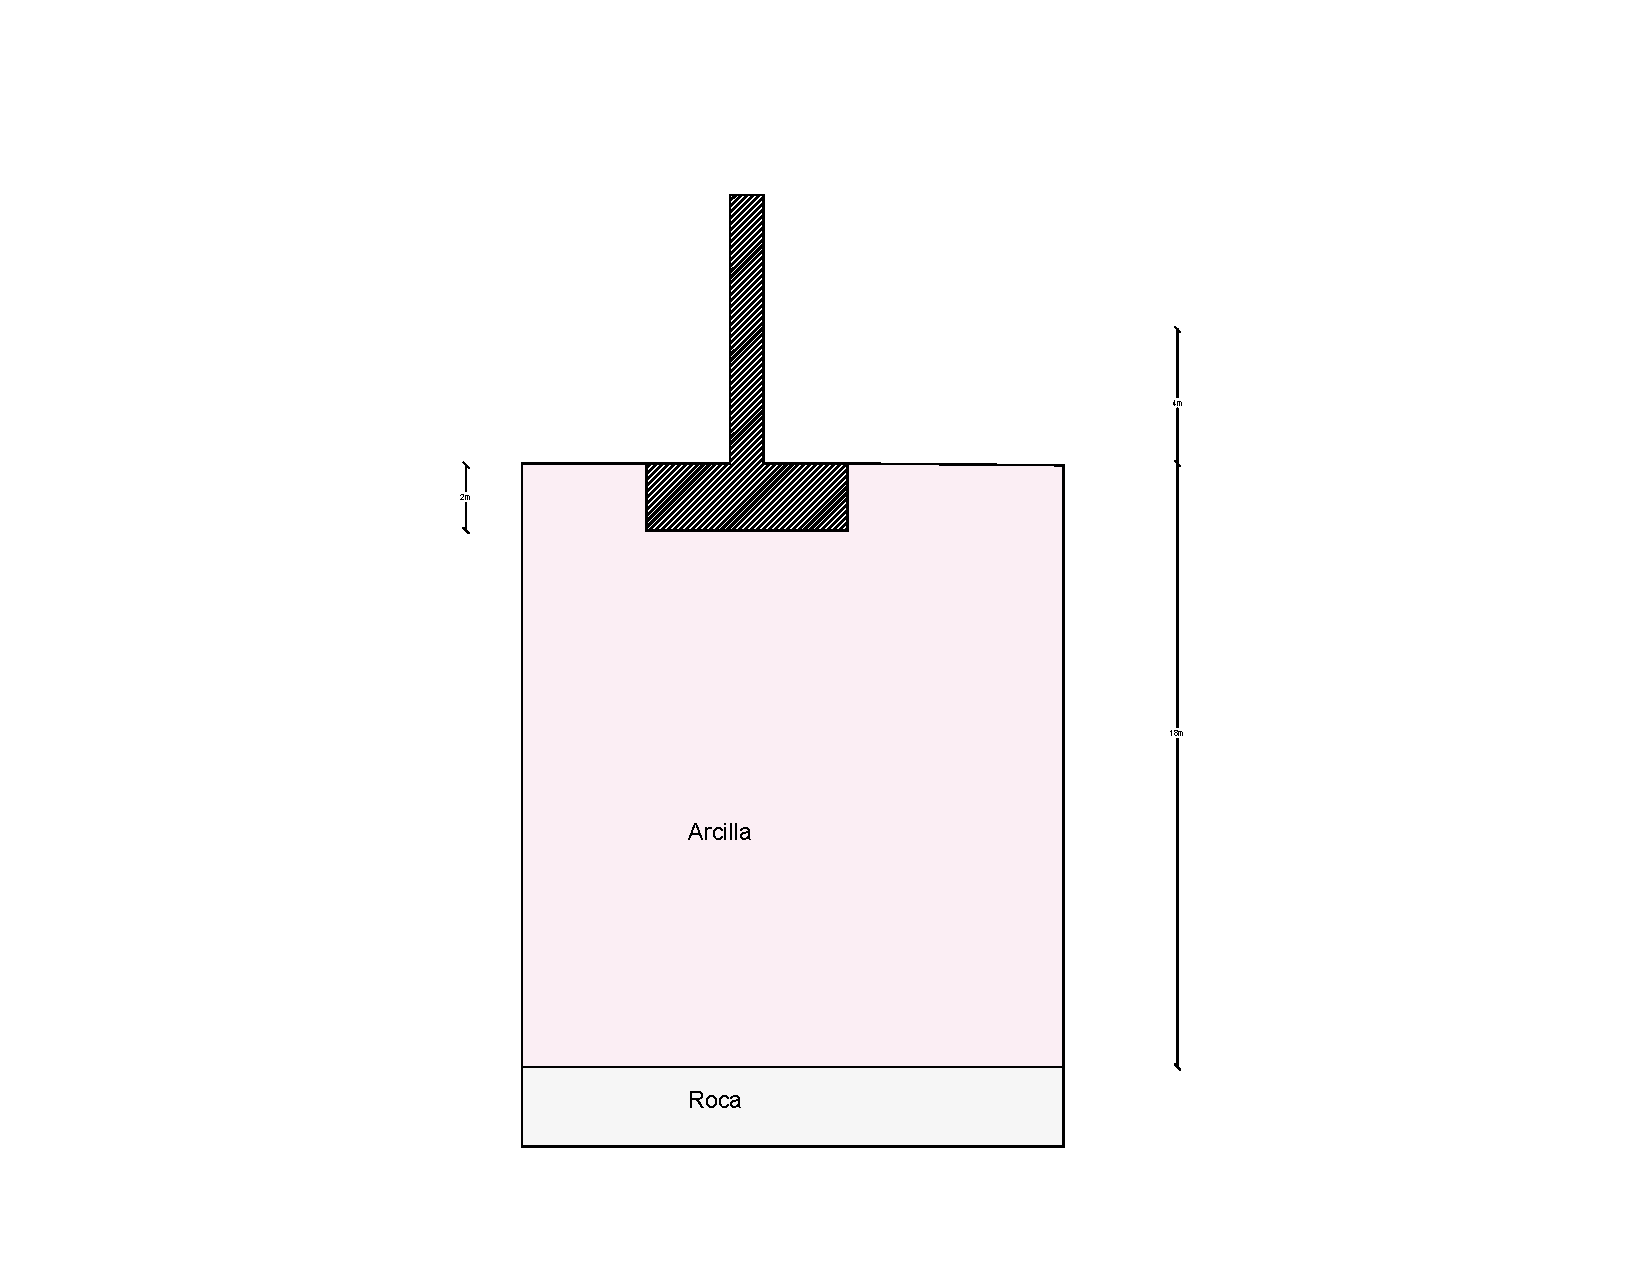
\includegraphics[width=0.5\textwidth]{img/cimentacion_larga}
		\caption{Cimentación cuadrada}
		\label{fig:ciment_larga}
	\end{figure}

	Al aplicarse rápidamente carga, nos situamos en condiciones drenadas. Analizaremos el problema en presiones totales y efectivas. Supondremos en ambos análisis $P = P_{peso-propio} + P_{peso aplicado}$

	\paragraph{Presiones totales} % (fold)
	\label{par:presiones_totales}
	
	\begin{multline}
		q_r = C_u N_c + \gamma_w H  = \frac{P + \gamma_w (H-h_b)(A_b - A_c)}{A_b}\\
		\Leftrightarrow P = C_u N_c A_b + \gamma_w (H- h_b) A_c + \gamma_w h_b A_b
	\end{multline}
	% paragraph presiones_totales (end)

	\paragraph{Presiones efectivas} % (fold)
	\label{par:presiones_efectivas}

	\begin{multline}
		q_r = C_u N_c  = \frac{P - \gamma_w h_b A_b - \gamma_w (H-h_b)(A_b - A_c)}{A_b}\\
		\Leftrightarrow P = C_u N_c A_b + \gamma_w (H- h_b) A_c + \gamma_w h_b A_b
	\end{multline}
	
	% paragraph presiones_efectivas (end)

	Luego tenemos 
	\[
		\Delta P = \gamma_w \Delta H A_c
	\]
}

\question{Si la carga se aplica lentamente (drenada), el valor de carga P con la que se alcanza la capacidad portante es de 12200T. ¿Con qué carga se alcanzaría la capacidad portante si el nivel del embalse estuviera 6m por encima de su nivel actual?}{
	A pesar de estar la capacidad portante en presiones efectivas, podemos trabajar en presiones totales o efectivas.
	\paragraph{Presiones totales} % (fold)
	\label{par:presiones_totales}
	\begin{multline}
		q_r^\prime + \gamma_w H = \frac{P  - \gamma_w (H-h_b)(A_b - A_c)}{A_b} \\
		\Leftrightarrow P = A_b q_r^\prime + \gamma_w H A_b  - \gamma_w (H-h_b)(A_b - A_c) \\
		\Leftrightarrow P = A_b q_r^\prime- \gamma_w H A_b h_b -  \gamma_w (H-h_b)A_c
	\end{multline}
	% paragraph presiones_efectivas (end)

	\paragraph{Presiones efectivas} % (fold)
	\label{par:presiones_efectivas}
	\begin{multline}
		q_r^\prime  = \frac{P -\gamma_w H A_b  - \gamma_w (H-h_b)A_c}{A_b} \\
		\Leftrightarrow P = A_b q_r^\prime- \gamma_w H A_b h_b -  \gamma_w (H-h_b)A_c
	\end{multline}
	% paragraph presiones_efectivas (end)

	Luego tenemos 
	\[
		\Delta P = -\gamma_w \Delta H A_c
	\]
}


\question{En el caso de la capacidad portante de una cimentación superficial ¿Qué caso es más crítico?
\begin{enumerate}
	\item Corto plazo 
	\item Largo plazo
\end{enumerate}}{
	El peor caso es a \emph{corto plazo} ya que como podemos ver en la Figure~\ref{fig:tensiones}, la trayectoria en tensiones totales (color verde) queda limitada por $C_u$. 
	\begin{figure}[H]
		\centering
		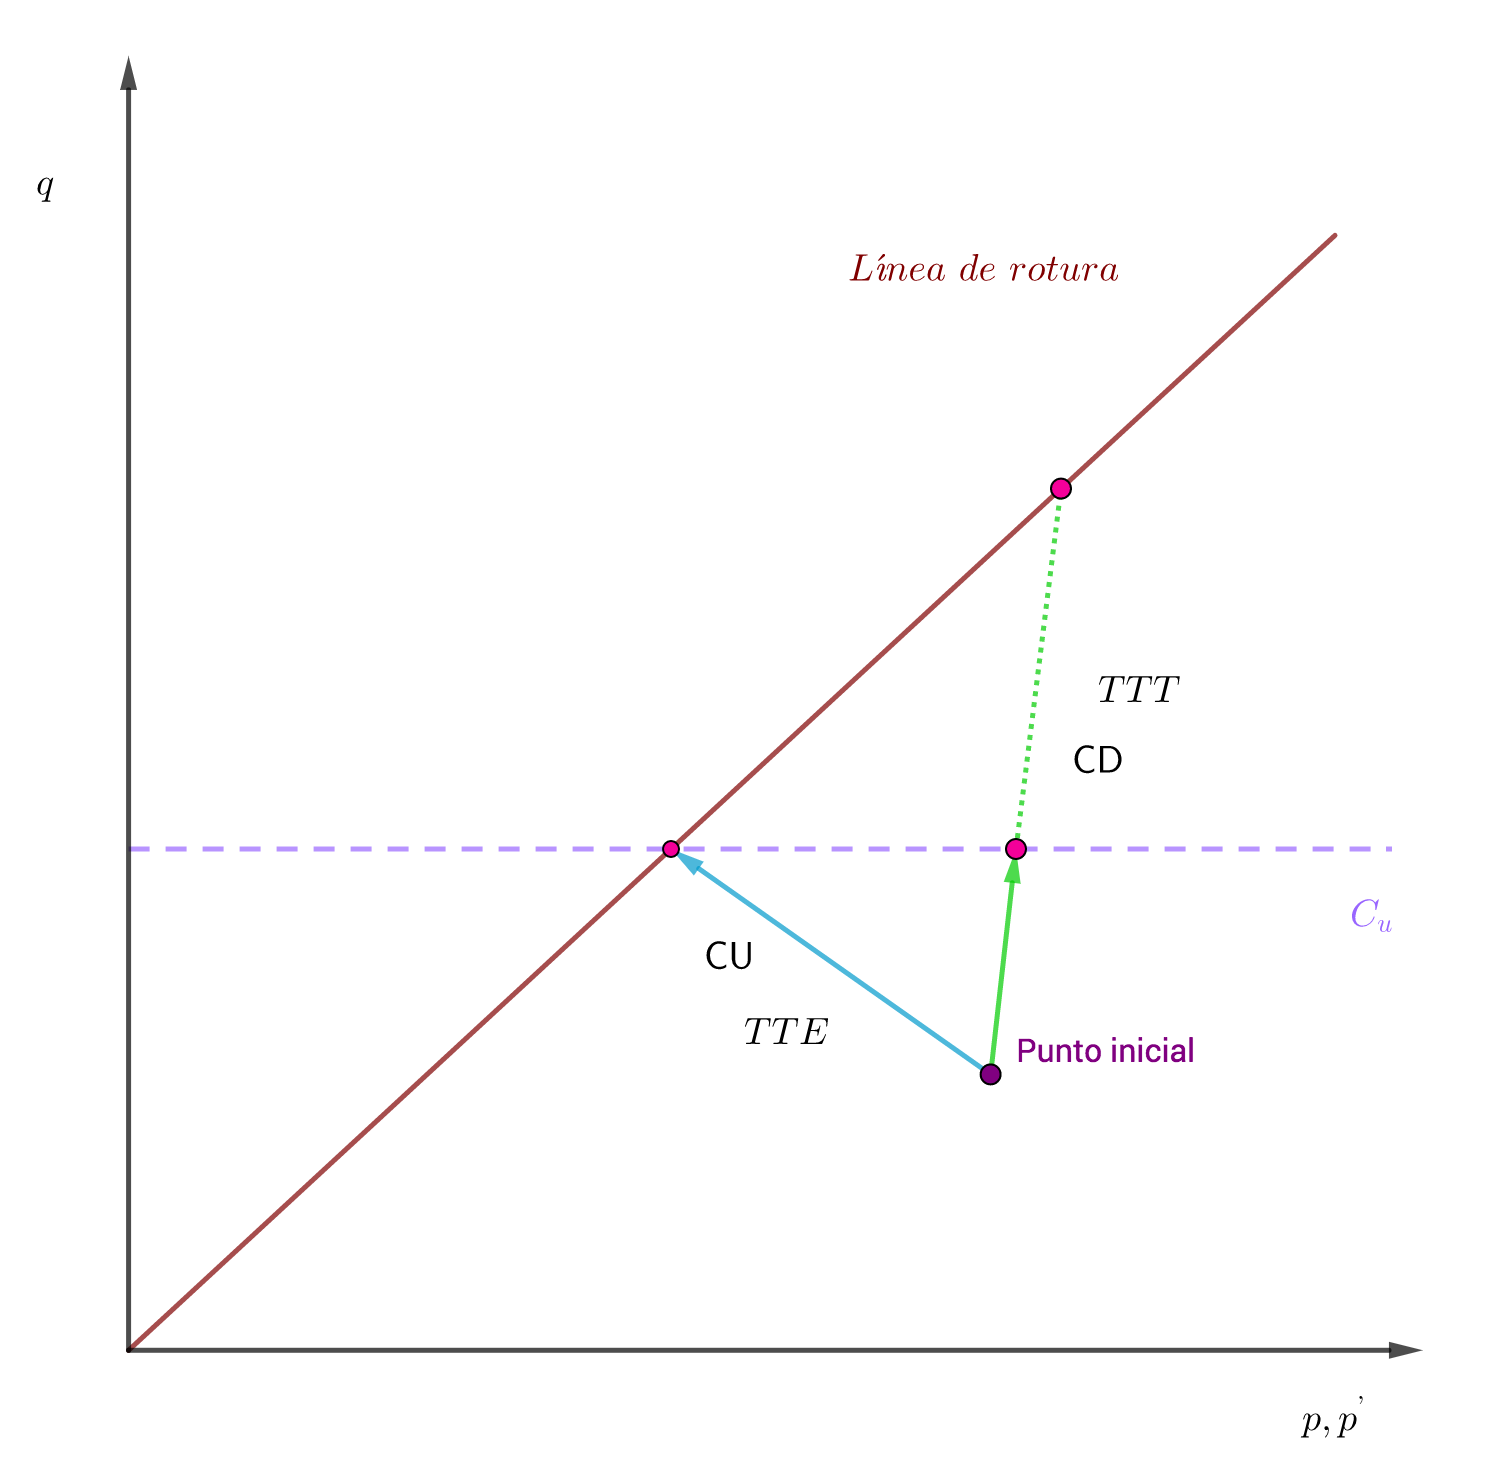
\includegraphics[width=0.5\textwidth]{img/trayectoria_tensiones}
		\caption{Trayectoria de tensiones }
		\label{fig:tensiones}
	\end{figure}
}

\question{Indica 3 posibles causas de deformación excesiva de una cimentación superficial no directamente relacionados con la carga aplicada}{
	\begin{enumerate}
		\item Levantamientos debidos a suelos expansivos o susceptibles a las heladas
		\item Deterioro del material de cimentación.
		\item Deformación por saturación de suelos colapsables (rellenos,loess)
		\item Deformación del terreno debido a excavaciones cercanas.
		\item Variación del NF
		\item Compactación del terreno por vibración, terremotos…
	\end{enumerate}
}

\question{La relación entre el asiento calculado por el método edométrico y por el método de Skempton es: 
\[
	S_{sb}= \mu S_{ed} = [A+\alpha (1-A)]S_{ed}
\]
Donde A es el parámetro de Skempton que depende de $\frac{z}{B}$. El valor de $\alpha$ para $\frac{z}{B}=0$ es 1. ¿Por qué?}{
	Una de las hipótesis del método edómetrico ($\epsilon_h = 0$) es que el incremento de presión intersticial es igual al incremento de presión vertical:
	\[
		\Delta u = \Delta \sigma_v
	\]
	El método de Skempton trata de mejorar esta aproximación introductiendo el parámetro $\mu = [A+\alpha (1-A)]$. Donde:
	\[
		\alpha \in[0,1] \propto 1-\frac{z}{B}
	\]
	En efecto si $\frac{z}{B}=0$, es decir la base es mucho mayor que la dimensión vertical del estrato (potencia), entonces nos situamos en condiciones edometricas y los asientos deben coincidir $\Rightarrow \alpha = 1$.
}


\question{Una placa de $\phi = 0,2m$ sometida a $10 T/m^2$ sufre un asiento de $0,2cm$. ¿Qué asiento se obtendrá al cargar una cimentación de $\phi = 1,2m$ y $20T/m^2$. Suponiendo suelo elástico-lineal?}{
	Tenemos $s \propto Q$ así pues:
	\[
		s_2 = s(2Q) = 2s(Q) = 2s_1
	\]
	Al tener un suelo elástico lineal $\frac{B}{s}=cte$, luego:
	\[
		s_3 = \frac{B_3}{B_2}s_2 
	\]	
	Luego mediante aplicación numerica $s_3 \approx 2,4cm$
}


\question{ En la práctica. ¿Esperarías que el asiento de la cimentación fuera mayor o menor que el calculado? ¿Por qué?}{
	La teoría elástico lineal no tiene en cuenta la variación del módulo elástico con la profundidad ($\frac{dE}{dz}>0$), luego es de esperar un asiento menor en la práctica.
}

\question{Las expresiones de la capacidad portante tienen la siguiente estructura (en terreno drenado):
\[
	q_r = cN_c + \frac{1}{2}\gamma B N_\gamma + qN_q
\]
}{
	\begin{enumerate}
	\item ¿A qué mecanismo de resistencia corresponde cada uno de los términos?
		\begin{enumerate}
			\item Contribución de la cohesión del suelo a la resistencia
			\item Efecto del peso
			\item Contribución de cargas sobre el plano de cimentación
		\end{enumerate}
	\item ¿Qué forma adopta en el caso de un terreno sumergido?
		En el caso de un terreno submergido hemos de tener en cuenta el efecto del empuje de Arquimedes, así pues podemos trabajar en tensiones efectivas:
		\begin{equation}
			\begin{cases}
				q_r^{’}=c^{’}N_c + \frac{1}{2}\gamma^{’} B N_\gamma + q^{’}N_q\\
				q_r =q_r^{’} + (p_w)_{base} 
			\end{cases}
		\end{equation}
	\item ¿Qué forma adopta en el caso de un análisis no drenado en tensiones totales $\phi = 0$
	Tenemos $N_q(\phi = 0)=1, N_\gamma(\phi = 0)=0$, luego:
	\[
		q_u = C_u N_c + q
	\]
	\item ¿Qué forma adoptaría q en el caso que el terreno de cimentación fuera exclusive agua?
	\begin{equation}
		\begin{cases}
			q_r =q_r^{’} + (p_w)_{base} = c^{’}N_c + \frac{1}{2}\gamma^{’} B N_\gamma + \gamma_w H_w, &\text{ drenado}\\
			q_r = C_uN_c + \gamma_w H_w,&\text{ no drenado}
		\end{cases}
	\end{equation}
\end{enumerate}
}

% section parte_2 (end)